\chapter{Meditation and the Sacred Mind}

This dialogue is not a blackboard lecture, yet it has a rigorous inner order. Krishnamurti does not derive equations; he derives consequences. A word is taken up, its hidden movement is exposed, and the next word follows from it: control, direction, will, decision, time, space, silence, energy, attention. We will keep that sequence intact. The displayed relations in this chapter are not formal psychological laws. They are compact note forms for the spoken inquiry, useful because they make visible the order in which the dialogue unfolds.

\section{Control, Direction, Will, Time}

Anderson begins by recalling the previous conversation on meditation, understanding, knowledge, and the flowering of a plant. The image matters: a flower does not force itself into order; it unfolds. Krishnamurti takes that opening and returns at once to control. If meditation is approached as control, then before we know what meditation is, we have already introduced a controller, a direction, and an end.

The first identity is the crucial one:

\begin{equation}
\text{controller} = \text{controlled}.
\end{equation}

This is not a technical equation. It is a denial of separation. The controller is not outside the field, operating on the field from a clean distance. It is one fragment trying to dominate other fragments. Once that is seen, control is no longer an innocent discipline; it is a circular movement inside fragmentation.

The chain that follows is the first conceptual derivation of the lecture:

\begin{equation}
\text{control}
\;\longrightarrow\;
\text{direction}
\;\longrightarrow\;
\text{will}
\;\longrightarrow\;
\text{decision, goal, achievement}
\;\longrightarrow\;
\text{time}.
\end{equation}

Control implies direction because control moves toward an end. Direction implies will because the end must be held and pursued. Will implies decision because something has been chosen as the thing to be carried out. Carrying out that decision has duration. Thus, by a series of small steps, meditation has been smuggled into time.

\begin{proposition}
In the inward field of this dialogue, psychological control contains the movement of time.
\end{proposition}

\begin{proof}
We keep only the lecture's own terms.
\begin{enumerate}
\item Control presupposes a controller directing what is controlled.
\item The controller is itself part of the controlled field.
\item Direction establishes an end or goal.
\item The end is carried by will and decision.
\item The movement from decision to achievement is duration.
\item Therefore psychological control carries time within it.
\end{enumerate}
\end{proof}

The result is simple but far-reaching. If meditation is something we practice in order to arrive somewhere, then meditation has become part of will. If it is part of will, it is part of time. Krishnamurti's question therefore becomes exact: what place has will in meditation and, since meditation is not separate from living, what place has will in life?

\begin{figure}
\centering
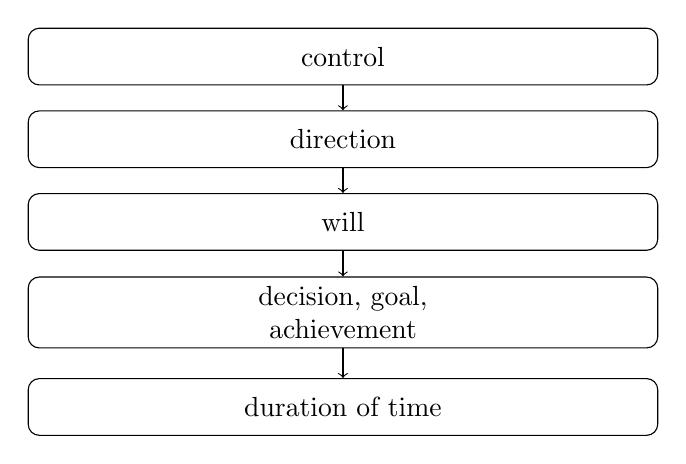
\begin{tikzpicture}
\node[draw, rounded corners, text width=0.64\linewidth, align=center, minimum height=0.72cm] (a) at (0,0) {control};
\node[draw, rounded corners, text width=0.64\linewidth, align=center, minimum height=0.72cm] (b) at (0,-1.05) {direction};
\node[draw, rounded corners, text width=0.64\linewidth, align=center, minimum height=0.72cm] (c) at (0,-2.10) {will};
\node[draw, rounded corners, text width=0.64\linewidth, align=center, minimum height=0.82cm] (d) at (0,-3.25) {decision, goal,\\ achievement};
\node[draw, rounded corners, text width=0.64\linewidth, align=center, minimum height=0.72cm] (e) at (0,-4.45) {duration of time};
\draw[->] (a) -- (b);
\draw[->] (b) -- (c);
\draw[->] (c) -- (d);
\draw[->] (d) -- (e);
\end{tikzpicture}
\caption{The opening sequence reconstructed from the transcript. It is a conceptual map, not a visible board diagram.}
\end{figure}

\subsection{Question \& Answer}

\paragraph{Question.}
Can there be a life without control, without will, and without direction?

\paragraph{Answer.}
The answer is not a rejection of practical intelligence. Krishnamurti immediately protects the field of knowledge. In ordinary life we need direction: to get home, to drive, to speak a language, to use technical knowledge. In that field, calculation, decision, and choice have their place.

The distinction is not between intelligence and passivity. It is between two fields:

\begin{table}
\centering
\begin{tabular}{p{0.43\linewidth} p{0.43\linewidth}}
\textbf{Field of knowledge} & \textbf{Inward field} \\
Direction, calculation, decision, and choice are necessary. & Psychological direction, will, and choice signal confusion. \\
Driving, language, technology, and ordinary navigation belong here. & Meditation, perception, attention, and inward order belong here. \\
Choice compares this with that. & Perception sees directly; action is not postponed by choice. \\
\end{tabular}
\caption{The working distinction between practical knowledge and inward perception.}
\end{table}

Inwardly, where there is choice there is confusion, because there is no perception. Where there is perception, choice has no place. We can write this as two complementary note relations:

\begin{align}
\text{choice without perception}
&\;\longrightarrow\;
\text{confusion}, \\
\text{perception}
&\;\longrightarrow\;
\text{action}.
\end{align}

Later the dialogue will make the second line even stronger: perception is action. For now, the important point is that meditation is not a controlled achievement. If it is controlled, it has already entered the chain of will and time.

\section{Knowledge, Disorder, and the False Division}

Anderson presses the distinction from another angle. Will seems valid in relation to know-how. Decision and choice belong to the ordinary career of knowledge. Krishnamurti agrees: direction belongs there, and so does calculation. But the confusion begins when that movement is brought into the inward field.

This is why the lecture does not permit an easy split between the practical and the spiritual. One might think: I can be efficient in knowledge and inwardly disordered; I can succeed outwardly and fail inwardly. Krishnamurti's reply is sharper. If there is not order inwardly, the outward action is also touched by disorder. The division between inner and outer is itself a product of thought.

So the distinction is functional, not metaphysical. Knowledge has its proper place. But when the structure of knowledge--direction, comparison, choice, achievement--is made into the structure of meditation, the mind merely extends confusion under a more serious name.

The lecture then returns to the earlier question with more force. Meditation covers the whole field of living, not one segment of it. If life cannot be lived without psychological control, will, direction, and achievement, then what is called meditation has no meaning. It becomes another escape: gurus, entertainments, practices, religious circuses. The repetition is deliberate. Krishnamurti is not making a quick anti-practice remark; he is showing why practice belongs to the very movement under examination.

Anderson offers a classical formulation of will as desire made reasonable. Krishnamurti accepts only what is useful in it: if desire and will are watched as they flower, then in the watching they lose vitality and wither. The image of flowering returns, but now it has become a methodless observation. One does not suppress will. One observes its movement.

\begin{equation}
\text{choiceless awareness of desire, control, will}
\;\longrightarrow\;
\text{loss of vitality in that movement}.
\end{equation}

The conclusion is not imposed. It appears as the movement is watched: there is no control.

\section{From Direction to Space}

From that ending of control, Krishnamurti makes the next pivot: direction means space. The word initially sounds unexpected. He does not begin by defining inward space. He begins with ordinary space: mountains need space, trees need space, flowers need space. Human beings, crowded into apartments, cities, repetitions of thought, fear, sorrow, and national identity, have less and less space. The point is concrete before it becomes inward.

Then comes the inward question: can the mind have space?

The earlier chain now reappears in a new form:

\begin{equation}
\text{direction}
\;\longrightarrow\;
\text{time}
\;\longrightarrow\;
\text{no inward space}.
\end{equation}

If the mind is occupied, filled with family, business, God, pleasure, fear, experience, or knowledge as thought, there is no space. Again, the terms should remain ordinary. Krishnamurti is not asking whether these things ever arise. He is asking what happens when occupation fills the whole field.

\begin{equation}
\text{occupation by thought and knowledge}
\;\longrightarrow\;
\text{no space}.
\end{equation}

Thought then creates a small enclosure around itself: me and you, we and they. The self lives in that little space. To move out of it appears as terror, anxiety, or the fear of not-being, because being has been identified with that enclosure.

\begin{definition}
Inward space, in this lecture, is not a private mental possession. It is the ending of the little space made by thought around the self.
\end{definition}

This gives a precise meaning to the statement that thought can never give space. Thought can make an enclosure and call it mine; it cannot give the open space that is not mine or yours. Meditation is therefore described as the freeing of the mind from its content as consciousness.

\begin{figure}
\centering
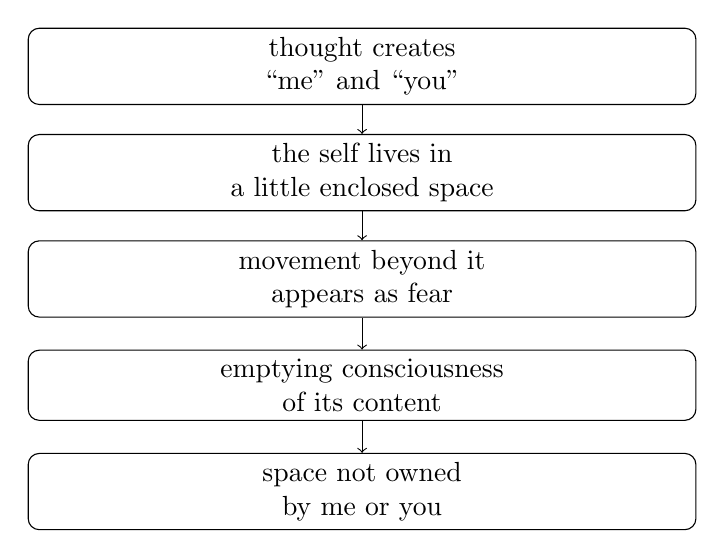
\begin{tikzpicture}
\node[draw, rounded corners, text width=0.68\linewidth, align=center, minimum height=0.8cm] (a) at (0,0) {thought creates\\ ``me'' and ``you''};
\node[draw, rounded corners, text width=0.68\linewidth, align=center, minimum height=0.8cm] (b) at (0,-1.35) {the self lives in\\ a little enclosed space};
\node[draw, rounded corners, text width=0.68\linewidth, align=center, minimum height=0.8cm] (c) at (0,-2.70) {movement beyond it\\ appears as fear};
\node[draw, rounded corners, text width=0.68\linewidth, align=center, minimum height=0.8cm] (d) at (0,-4.05) {emptying consciousness\\ of its content};
\node[draw, rounded corners, text width=0.68\linewidth, align=center, minimum height=0.8cm] (e) at (0,-5.40) {space not owned\\ by me or you};
\draw[->] (a) -- (b);
\draw[->] (b) -- (c);
\draw[->] (c) -- (d);
\draw[->] (d) -- (e);
\end{tikzpicture}
\caption{A transcript-based map of the movement from thought's enclosed space to inward space.}
\end{figure}

The outward landscape cannot supply this inward space. One may go to the country, take a vacation, or move from one setting to another, but if occupation continues, one goes from one enclosure to another. Inward space appears when what has to be done is done and is not carried on as psychological residue.

\section{Space Means Silence}

The next movement is short and exact: space means silence. But the word silence has to be protected. Krishnamurti does that by ruling out the common substitutes. Silence is not the interval between two noises. It is not the cessation of noise. It is not something thought has made. It is not induced by practice. It is not the atmosphere of a church or temple, however impressive that atmosphere may be.

A compact negative definition keeps the distinctions visible:

\begin{align}
\text{silence} &\neq \text{interval between noises}, \\
\text{silence} &\neq \text{cessation of noise}, \\
\text{silence} &\neq \text{a state produced by thought}, \\
\text{silence} &\neq \text{a result induced by practice}.
\end{align}

This exclusion is part of the teaching. If silence is produced by thought, it remains within thought. If it is induced by practice, it remains within will and time. If it is merely an interval, it is still measured by the noises around it.

\subsection{Question \& Answer}

\paragraph{Question.}
Can silence operate in daily life while we still live in the necessary field of knowledge?

\paragraph{Answer.}
Krishnamurti says that it can. The answer is not withdrawal from knowledge. We still speak, work, calculate, remember, and perform technical actions. The question is whether the field of knowledge and silence can move together without division. Anderson hears the difficulty, and Krishnamurti gives the image of two rivers flowing together in balance.

The note form is:

\begin{equation}
\text{practical knowledge}
\;+\;
\text{silence without division}
\;\longrightarrow\;
\text{harmony in living}.
\end{equation}

If this were impossible, then we would be confined to the field of knowledge. Krishnamurti insists that it is possible, and that insistence is the bridge to the next question. If silence can operate in daily life, what is creation?

\section{Creation, Measure, and the Immeasurable}

Creation is introduced late because it depends on what has already been unfolded. If creation is discussed before control, space, and silence have been understood, it easily becomes expression: painting, writing, composing, making, producing, pressing something out of oneself. Anderson notices the literal pressure in the word expression, and Krishnamurti accepts the danger. A person may be in inward tension and produce a book out of that tension. That may be expression, but it is not the creation being asked about here.

Creation, in this movement of the dialogue, is creation in living. The image returns: flowering in which the flower does not know that it is flowering. This matters because the same image has already described desire and will when they are observed without choice. Flowering is not self-improvement. It is the full exposure of a movement, and in that exposure the movement changes.

Then the conversation turns to a more exact obstacle:

\begin{equation}
\text{thought} = \text{measure}.
\end{equation}

If thought is measure, then the search for the immeasurable through thought has no meaning. Thought may assert the eternal, the unnameable, the sacred, or God, but such assertion remains a projection or speculation. The measured cannot arrive at the immeasurable by extending itself.

\begin{proposition}
Within this dialogue, the immeasurable is not reached by a movement of thought.
\end{proposition}

\begin{proof}
\begin{enumerate}
\item Thought is named as measure.
\item A search conducted by thought remains a measured movement.
\item A measured movement cannot produce the immeasurable as its achievement.
\item Therefore the search for the immeasurable through thought has no meaning.
\end{enumerate}
\end{proof}

This does not deny the immeasurable. It denies the route of assertion, speculation, and thought-made religion. The question is restated more carefully: when the mind is utterly silent, what is the immeasurable?

\section{Energy, the Sacred, and Secondary Powers}

In silence, Krishnamurti says, energy is not dissipated. The word energy must stay within the discipline of the transcript. It is not a physical variable. It names what is gathered when conflict, control, reaching, searching, asking, demanding, waiting, and praying are absent.

\begin{equation}
\text{silence}
-
\{\text{conflict},\text{control},\text{seeking},\text{asking},\text{praying}\}
\;\longrightarrow\;
\text{gathered energy}.
\end{equation}

And later the relation is made even more compact:

\begin{equation}
\text{attention}
\;\approx\;
\text{gathering of all energy}.
\end{equation}

The approximation sign is only a note-writing convention. Krishnamurti's phrase is not a mathematical equivalence. It means that attention is not scattered effort; it is the gathered seriousness of a mind not wasting itself in conflict.

\begin{figure}
\centering
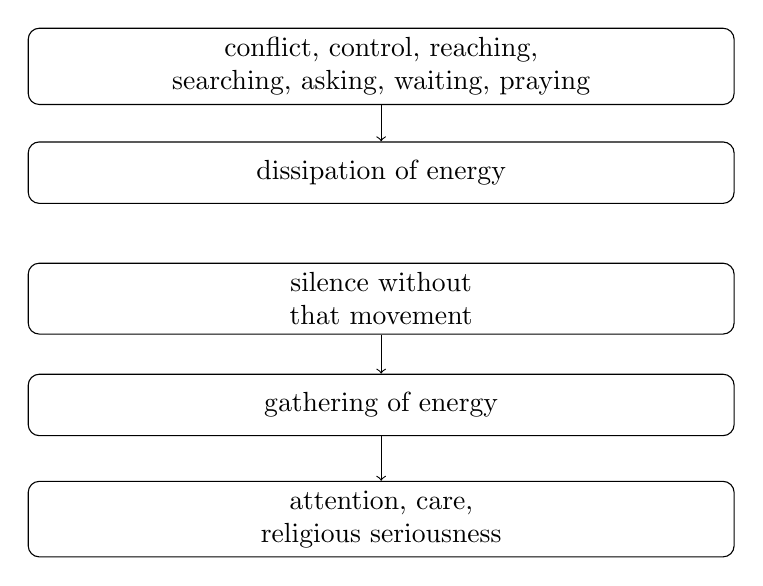
\begin{tikzpicture}
\node[draw, rounded corners, text width=0.72\linewidth, align=center, minimum height=0.86cm] (a) at (0,0) {conflict, control, reaching,\\ searching, asking, waiting, praying};
\node[draw, rounded corners, text width=0.72\linewidth, align=center, minimum height=0.78cm] (b) at (0,-1.35) {dissipation of energy};
\node[draw, rounded corners, text width=0.72\linewidth, align=center, minimum height=0.86cm] (c) at (0,-2.95) {silence without\\ that movement};
\node[draw, rounded corners, text width=0.72\linewidth, align=center, minimum height=0.78cm] (d) at (0,-4.30) {gathering of energy};
\node[draw, rounded corners, text width=0.72\linewidth, align=center, minimum height=0.86cm] (e) at (0,-5.75) {attention, care,\\ religious seriousness};
\draw[->] (a) -- (b);
\draw[->] (c) -- (d);
\draw[->] (d) -- (e);
\end{tikzpicture}
\caption{A transcript-based reconstruction of the movement from dissipation to gathered energy.}
\end{figure}

That gathered silence is called sacred. Krishnamurti immediately distinguishes it from the sacred thing invented by thought. The sacred is not an image, word, doctrine, or object set apart by belief. When the mind itself becomes sacred, he says, it opens the door to what is immeasurably sacred. Religion, in this use, is not belief but a way of living that touches speech, conduct, relationship, and care.

Then the lecture tests a dangerous by-product. When energy is gathered, powers may appear: healing, miracles, extrasensory capacities. Krishnamurti does not build a doctrine from them. He says they are secondary and dangerous because they can strengthen the self.

\begin{equation}
\text{talent or power}
\;\longrightarrow\;
\text{importance of me}
\;\longrightarrow\;
\text{position, money, worship}.
\end{equation}

The old story about learning to walk on water makes the point without abstraction: if there is a boat, the miraculous display is beside the point. The religious mind does not touch the secondary power as identity. It puts it away.

Anderson then returns to energy and pattern. He suggests that our gaze should move from the pattern to the energy itself. Krishnamurti accepts the word energy and turns it toward love: the religious summation of energy is love, compassion, and care operating in daily life. But when love is dragged back into the track of knowledge, it becomes sensation, and therefore is no longer love in the sense being discussed.

\section{Prayer, Books, Attention, and the Ending of Suffering}

The last major test is prayer. Anderson asks because convention joins prayer and meditation. Krishnamurti answers directly: prayer, as petition, has no place in meditation. Petition means asking, begging, supplicating. It arises when one does not understand, when one is in conflict, sorrow, violence, loss, or desire for achievement.

\subsection{Question \& Answer}

\paragraph{Question.}
If prayer as petition has no place in meditation, is there any use of prayer that belongs with this inquiry?

\paragraph{Answer.}
The dialogue does not develop a positive technique of prayer. It removes petition. If there is no petition, there is no asking. If there is no asking, one can look. Anderson names this quietude; Krishnamurti calls it real peace.

\begin{equation}
\text{no petition}
\;\longrightarrow\;
\text{no asking}
\;\longrightarrow\;
\text{looking}
\;\longrightarrow\;
\text{real peace}.
\end{equation}

The examples are deliberately plain: praying for a refrigerator, praying for peace while living violently, praying for one's country while sustaining division. Petition reproduces the very disorder from which it asks to be rescued.

From prayer the conversation turns to books and teachers. Books have become important; the mind becomes second-hand through what others have said about reality. The issue is not literacy or learning in the practical field. The issue is whether a mind filled with second-hand authority can come upon what is original. Krishnamurti refuses the sequence of acquiring, rejecting, and then receiving. Why go through those stages? Why not look?

The teacher also dissolves under the same pressure. No teacher can give this, because the teacher and the taught are not finally separate in the way dependency imagines. The disciple is the teacher. The statement belongs with the earlier identity of controller and controlled: the division that promises rescue is itself part of the structure to be seen.

The dialogue then returns to seriousness. Meditation is not one activity among other activities. It means attention and care: care for children, neighbor, country, earth, trees, animals. Seriousness brings attention, care, and responsibility. One does not proceed through a ladder of stages; one sees.

The final chain is the simplest:

\begin{equation}
\text{perception}
\;\longrightarrow\;
\text{action}
\;\longrightarrow\;
\text{wisdom}
\;\longrightarrow\;
\text{ending of suffering}.
\end{equation}

Wisdom is not callousness. It is the ending of suffering. Suffering ends not by refusal, rationalization, escape, or the decision to go beyond it, but by being seen. It flowers in choiceless awareness, and as it flowers it withers. Here the opening image returns one last time: order is not forced; the movement is understood as it unfolds.

Anderson speaks of energy free to pattern itself or not to pattern itself. Krishnamurti's final formulation brings the whole lecture back to time:

\begin{equation}
\text{silence}
\;\longrightarrow\;
\text{time stops}.
\end{equation}

This is not a technical claim about clock time. It is the culmination of the opening chain. Control brought direction, will, decision, and time. Silence is the ending of that movement. In that sense, time stops.

\section{Summary}

The chapter has followed the lecture's own sequence. Control reveals direction; direction reveals will; will reveals decision and time. The first essential distinction is between practical knowledge, where direction and choice are necessary, and inward perception, where choice indicates confusion and action follows seeing without interval.

The inquiry then turns from time to space. Thought creates a little enclosure around the self; occupation fills the mind; inward space appears only when consciousness is emptied of its content. Space becomes silence, but silence is not acoustic quiet, not practice, not thought-made stillness, and not an interval between noises.

From silence the dialogue moves to creation, the immeasurable, energy, and the sacred. Thought is measure, so thought cannot reach the immeasurable by pursuit or assertion. In silence, energy is no longer dissipated by conflict, control, seeking, asking, and praying. That gathered energy is attention, care, and religious seriousness. The chapter closes where it began: if control is time, then silence is the ending of that movement. In silence, time stops.